% !TeX program = pdflatex
\documentclass[aspectratio=169,10pt]{beamer}
\usetheme{metropolis}
\metroset{block=fill, numbering=fraction, progressbar=frametitle}

% ============================================================
% PACKAGES
% ============================================================
\usepackage[utf8]{inputenc}
\usepackage[T1]{fontenc}
\usepackage{amsmath}
\usepackage{amsfonts}
\usepackage{amssymb}
\usepackage{xcolor}
\usepackage{tikz}
\usetikzlibrary{shapes,arrows,arrows.meta,positioning,fit,backgrounds,calc,shadows,decorations.pathreplacing}
\usepackage{pgfplots}
\pgfplotsset{compat=1.18}
\usepackage{booktabs}
\usepackage{colortbl}
\usepackage{array}
\usepackage{mdframed}

% ============================================================
% PREMIUM COLOR SYSTEM — Enterprise Palette
% ============================================================
\definecolor{primaryDark}{RGB}{31,58,95}      % #1F3A5F
\definecolor{primary}{RGB}{47,93,159}         % #2F5D9F
\definecolor{primaryLight}{RGB}{100,140,200}
\definecolor{accentTeal}{RGB}{24,169,153}     % #18A999
\definecolor{accentEmerald}{RGB}{47,191,113}  % #2FBF71
\definecolor{accentOrange}{RGB}{244,162,97}   % #F4A261
\definecolor{accentOrangeDark}{RGB}{230,130,60}
\definecolor{bgMain}{RGB}{246,248,251}        % #F6F8FB
\definecolor{bgCard}{RGB}{255,255,255}        % #FFFFFF
\definecolor{bgLayer1}{RGB}{240,244,250}      % Soft API Layer
\definecolor{bgLayer2}{RGB}{240,248,246}      % Soft Intelligence Layer
\definecolor{bgLayer3}{RGB}{252,246,240}      % Soft Infrastructure Layer
\definecolor{bgHighlight}{RGB}{245,248,250}
\definecolor{borderLight}{RGB}{220,227,236}   % #DCE3EC
\definecolor{borderMedium}{RGB}{180,190,200}
\definecolor{textDark}{RGB}{28,32,38}
\definecolor{textMedium}{RGB}{80,88,100}
\definecolor{textLight}{RGB}{130,140,155}

% ============================================================
% BEAMER CONFIGURATION
% ============================================================
\setbeamercolor{background canvas}{bg=bgMain}
\setbeamercolor{normal text}{fg=textDark}
\setbeamercolor{title}{fg=primaryDark}
\setbeamercolor{frametitle}{fg=primaryDark}
\setbeamertemplate{itemize item}{\color{primary}$\blacktriangleright$}
\setbeamertemplate{itemize subitem}{\color{accentTeal}$\triangleright$}
\setbeamertemplate{navigation symbols}{}

% ============================================================
% PREMIUM TITLE STYLE — Keynote Quality
% ============================================================
\makeatletter
\setbeamertemplate{frametitle}{%
  \vspace{0.25cm}
  \begin{flushleft}
    {\color{primaryDark}\Large\bfseries\insertframetitle\par}
    \vspace{0.06cm}
    {\color{accentTeal}\rule{0.18\textwidth}{2.5pt}}\par
  \end{flushleft}
  \vspace{0.05cm}
}
\makeatother

% ============================================================
% PREMIUM CARD ENVIRONMENTS
% ============================================================
\newenvironment{herocard}[1][0.98\textwidth]{%
  \begin{center}
  \begin{mdframed}[
    linewidth=0.5pt,
    linecolor=borderLight,
    backgroundcolor=bgCard,
    roundcorner=8pt,
    shadow=true,
    shadowsize=4pt,
    shadowcolor=black!6,
    innertopmargin=8pt,
    innerbottommargin=8pt,
    innerleftmargin=12pt,
    innerrightmargin=12pt
  ]
  \begin{minipage}{#1}
}{%
  \end{minipage}
  \end{mdframed}
  \end{center}
}

\newenvironment{card}[1][0.98\textwidth]{%
  \begin{center}
  \begin{mdframed}[
    linewidth=0.5pt,
    linecolor=borderLight,
    backgroundcolor=bgCard,
    roundcorner=6pt,
    shadow=true,
    shadowsize=3pt,
    shadowcolor=black!5,
    innertopmargin=8pt,
    innerbottommargin=8pt,
    innerleftmargin=10pt,
    innerrightmargin=10pt
  ]
  \begin{minipage}{#1}
}{%
  \end{minipage}
  \end{mdframed}
  \end{center}
}

\newenvironment{smallcard}[1][0.48\textwidth]{%
  \begin{mdframed}[
    linewidth=0.4pt,
    linecolor=borderLight,
    backgroundcolor=bgCard,
    roundcorner=5pt,
    shadow=true,
    shadowsize=2pt,
    shadowcolor=black!4,
    innertopmargin=5pt,
    innerbottommargin=5pt,
    innerleftmargin=7pt,
    innerrightmargin=7pt
  ]
  \begin{minipage}{#1}
}{%
  \end{minipage}
  \end{mdframed}
}

% ============================================================
% TIKZ STYLES — Enterprise-Grade Diagrams
% ============================================================
\tikzset{
  % Grouped Zones (visual depth layer)
  zoneLayer/.style={
    draw=borderLight!90, fill=#1, rounded corners=10pt, line width=0.8pt,
    drop shadow={shadow xshift=2.0pt, shadow yshift=-2.0pt, opacity=0.05}
  },
  % Base Elevating Cards (Flat White Services)
  cardNode/.style={
    rectangle, draw=borderLight, fill=white, rounded corners=6pt, line width=0.6pt,
    minimum width=2.2cm, minimum height=0.65cm, align=center, font=\scriptsize\bfseries\color{textDark},
    drop shadow={shadow xshift=1.2pt, shadow yshift=-1.2pt, opacity=0.08}
  },
  % Primary Active Cards (Muted Blue Corporate Fills)
  cardPrimary/.style={
    rectangle, draw=primary!70, fill=primary!4, rounded corners=6pt, line width=1.0pt,
    minimum width=2.4cm, minimum height=0.75cm, align=center, font=\scriptsize\bfseries\color{primaryDark},
    drop shadow={shadow xshift=1.5pt, shadow yshift=-1.5pt, opacity=0.14}
  },
  % Teal Subsystem Cards (Modern Caching/Telemetry Accent)
  cardTeal/.style={
    rectangle, draw=accentTeal!75, fill=accentTeal!4, rounded corners=6pt, line width=1.0pt,
    minimum width=2.4cm, minimum height=0.75cm, align=center, font=\scriptsize\bfseries\color{primaryDark},
    drop shadow={shadow xshift=1.5pt, shadow yshift=-1.5pt, opacity=0.12}
  },
  % Dominant Highlight Cards (Glow Innovation Core)
  cardHighlight/.style={
    rectangle, draw=accentOrangeDark!95, fill=accentOrange!12, rounded corners=8pt, line width=1.6pt,
    minimum width=2.8cm, minimum height=0.85cm, align=center, font=\small\bfseries\color{primaryDark},
    drop shadow={shadow xshift=2.0pt, shadow yshift=-2.0pt, opacity=0.22}
  },
  % Soft Secondary Nodes (Helper microservices)
  cardSecondary/.style={
    rectangle, draw=borderLight, fill=bgMain, rounded corners=5pt, line width=0.5pt,
    minimum width=2.0cm, minimum height=0.58cm, align=center, font=\tiny\bfseries\color{textMedium},
    drop shadow={shadow xshift=0.8pt, shadow yshift=-0.8pt, opacity=0.04}
  },
  % Routing Arrows
  flowArrow/.style={
    ->, >=Stealth, thick, primary!70, shorten >=2pt, shorten <=2pt, line width=1.0pt
  },
  flowArrowDashed/.style={
    ->, >=Stealth, dashed, thick, primaryLight!80, shorten >=2pt, shorten <=2pt, line width=0.8pt
  },
  flowArrowAccent/.style={
    ->, >=Stealth, very thick, accentTeal!90, shorten >=2pt, shorten <=2pt, line width=1.2pt
  },
  % Legacy Aliases for Backward Compatibility
  layerAPI/.style={zoneLayer={bgLayer1}, minimum width=10cm, minimum height=0.85cm},
  layerIntel/.style={zoneLayer={bgLayer2}, minimum width=10cm, minimum height=0.85cm},
  layerInfra/.style={zoneLayer={bgLayer3}, minimum width=10cm, minimum height=0.85cm},
  sublayer/.style={cardNode, minimum width=2.2cm, minimum height=0.6cm, font=\small},
  arrow/.style={flowArrow, primary!50},
  heroarrow/.style={flowArrowAccent, primary!60},
  nodeCircle/.style={circle, draw=primary!50, fill=bgCard, minimum size=1cm, align=center, font=\footnotesize, drop shadow},
  pipeline/.style={cardNode, minimum width=1.8cm, minimum height=0.7cm, font=\small},
  pipelineTint/.style={cardNode, draw=borderLight, fill=bgHighlight, minimum width=1.8cm, minimum height=0.7cm, font=\small\bfseries},
  pipelineHighlight/.style={cardHighlight, minimum width=1.8cm, minimum height=0.7cm, font=\small\bfseries},
  pipelinePrimary/.style={cardPrimary, minimum width=2.8cm, minimum height=0.95cm, font=\small\bfseries},
  pipelineSecondary/.style={cardSecondary, minimum width=2.3cm, minimum height=0.78cm, font=\footnotesize},
  pipelineAccent/.style={cardTeal, minimum width=2.8cm, minimum height=1.0cm, font=\small\bfseries},
  heroNode/.style={cardHighlight, minimum width=3.6cm, minimum height=1.3cm, font=\small\bfseries}
}

% ============================================================
% SECTION TRANSITION SLIDES — Cinematic Widescreen Transitions
% ============================================================
\newcommand{\sectiontransition}[3]{%
  {
  \setbeamercolor{background canvas}{bg=primaryDark}
  \begin{frame}[plain]
  \vspace{1.5cm}
  \begin{flushleft}
    {\color{accentOrange}\fontsize{42}{46}\selectfont\bfseries #1}\\[0.2cm]
    {\color{white}\Huge\bfseries #2}\\[0.3cm]
    {\color{accentTeal}\rule{0.35\textwidth}{3.0pt}}\\[0.5cm]
    {\color{bgHighlight}\large\itshape ``#3''}
  \end{flushleft}
  \end{frame}
  }
}

% ============================================================
% TITLE SLIDE
% ============================================================
\title[MandiSense AI]{\textbf{MandiSense AI}\\ An Adaptive Agentic Agricultural Decision Intelligence Platform}
\subtitle{Multi-Agent Forecasting · Volatility Reasoning · Explainable Operational Cognition}
\author{\textbf{Agricultural Intelligence Systems Lab}}
\date{IEEE/ACM Conference on AI Systems Engineering · 2026}

\begin{document}

{
\setbeamercolor{background canvas}{bg=white}
\begin{frame}[plain]
\titlepage
\end{frame}
}

% ============================================================
% SECTION 01: RESEARCH FOUNDATION
% ============================================================
\sectiontransition{01}{Research Foundation}{Understanding the Need for Adaptive Agricultural Intelligence}

% --- SLIDE 2: PROBLEM BACKGROUND ---
\begin{frame}{Problem Background — Market Volatility and Operational Fragmentation}
\begin{herocard}
\begin{itemize}
    \small
    \item Agricultural commodity markets exhibit extreme regional volatility driven by weather, logistics, and policy shocks.
    \item Decision makers rely on delayed forecasts, disconnected supply chain signals, and inconsistent mandi data.
    \item Existing systems were designed for historical batch delivery, not live market intelligence.
    \item The gap between model outputs and actionable advisory insights undermines farmer and trader trust.
    \item Without integrated operational cognition, risk management and price discovery remain fragmented.
\end{itemize}
\end{herocard}
\end{frame}

% --- SLIDE 3: PROBLEM STATEMENT ---
\begin{frame}{Problem Statement — Why MandiSense AI?}
\begin{herocard}
\begin{itemize}
    \small
    \item Current agricultural intelligence platforms fail to support adaptive decision-making under rapid regime shifts.
    \item Static forecasting and monolithic pipelines cannot respond to volatile mandi behavior in real time.
    \item There is no end-to-end solution that combines multi-agent prediction, volatility-aware fusion, explainability, and resilient backend operations.
    \item The problem is not only prediction accuracy; it is the lack of operationally trustworthy intelligence for market actors.
    \item MandiSense AI is designed to close this gap with production-grade adaptive agricultural cognition.
\end{itemize}
\end{herocard}
\end{frame}

% --- SLIDE 4: THE AGRICULTURAL DECISION CRISIS ---
\begin{frame}{The Agricultural Decision Crisis}
\begin{herocard}
\begin{columns}[T]
\column{0.5\textwidth}
\centering
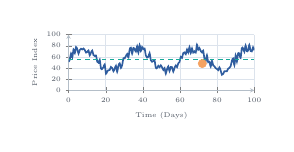
\begin{tikzpicture}[scale=0.5]
\begin{axis}[
    width=6.3cm, height=3.0cm,
    xlabel={Time (Days)}, ylabel={Price Index},
    xmin=0, xmax=100, ymin=0, ymax=100,
    axis lines=left,
    tick label style={font=\tiny, color=textMedium},
    label style={font=\tiny, color=textMedium},
    axis line style={color=borderMedium},
    grid=both, grid style={color=borderLight, thin},
    domain=0:100, samples=150,
]
\addplot[primary, very thick, smooth] {55 + 20*sin(x*360/30) + 8*rand};
\addplot[accentTeal, thick, dashed] {55};
\addplot[accentOrange, only marks, mark=*, mark size=3] coordinates {(72, 48)};
\end{axis}
\end{tikzpicture}
\column{0.4\textwidth}
\raggedright
\begin{itemize}\setlength{\itemsep}{0.5ex}\setlength{\parskip}{0pt}
    \scriptsize
    \item \color{accentOrange}\bfseries 40–60\% price swings within harvest cycles
    \item \bfseries 10,000+ markets, information asymmetry
    \item Fragmented intelligence systems limit real-time coordination
    \item Static forecasts ignore volatility regimes and shock events
    \item \bfseries 78\% of farmers distrust black-box models
\end{itemize}
\end{columns}
\end{herocard}
\vspace{0.1cm}
\centering{\color{accentTeal}\itshape\normalsize ``Where decisions are most critical, forecasting is least reliable.''}
\end{frame}

% --- SLIDE 5: LITERATURE SURVEY ---
\begin{frame}{Literature Survey — Comparative Landscape}
\begin{herocard}
\centering
\scriptsize
\begin{tabular}{p{1.8cm}|p{2.2cm}|p{2.2cm}|p{2.2cm}}
\toprule
\bfseries Approach & \bfseries Strength & \bfseries Limitation & \bfseries Missing Capability \\
\midrule
ARIMA / SARIMA & Transparent statistical baseline & Poor under non-stationary volatility & No adaptive regime awareness \\
\addlinespace
Static ML Ensemble & Combines multiple predictors & Fixed weights, delayed adaptation & No conflict-aware fusion \\
\addlinespace
Agricultural Forecast Systems & Domain-specific market features & Monolithic pipelines, little explainability & Lacks operational cognition and parallel reasoning \\
\addlinespace
Post-hoc XAI frameworks & Explainability on demand & Not integrated at runtime & No real-time decision intelligence \\
\bottomrule
\end{tabular}
\vspace{0.3cm}
\centering{\scriptsize\color{textMedium}The gap is not accuracy alone; it is the missing fusion of adaptive reasoning, explainability, and live operational infrastructure.}
\end{herocard}
\end{frame}

% --- SLIDE 4: GAP ---
\begin{frame}{Research Gap — From Legacy Forecasting to Operational Cognition}
\begin{herocard}
\centering
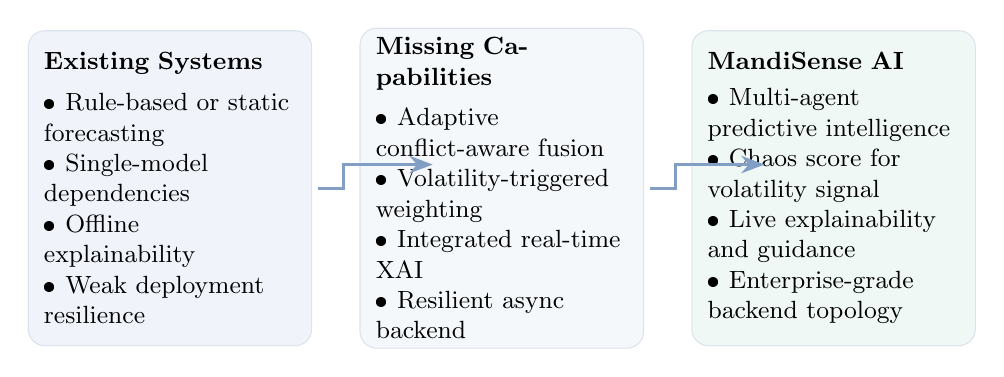
\begin{tikzpicture}[node distance=0.25cm, every node/.style={font=\small}]
\node[draw=borderLight, fill=bgLayer1, rounded corners=6pt, minimum width=3.6cm, minimum height=4.0cm, text width=3.2cm, align=left] (existing) {
  \textbf{Existing Systems}\vspace{0.2cm}
  \parbox{3.2cm}{\small\raggedright
    \textbullet\ Rule-based or static forecasting\\
    \textbullet\ Single-model dependencies\\
    \textbullet\ Offline explainability\\
    \textbullet\ Weak deployment resilience
  }
};
\node[draw=borderLight, fill=bgHighlight, rounded corners=6pt, right=0.6cm of existing, minimum width=3.6cm, minimum height=4.0cm, text width=3.2cm, align=left] (gap) {
  \textbf{Missing Capabilities}\vspace{0.2cm}
  \parbox{3.2cm}{\small\raggedright
    \textbullet\ Adaptive conflict-aware fusion\\
    \textbullet\ Volatility-triggered weighting\\
    \textbullet\ Integrated real-time XAI\\
    \textbullet\ Resilient async backend
  }
};
\node[draw=borderLight, fill=bgLayer2, rounded corners=6pt, right=0.6cm of gap, minimum width=3.6cm, minimum height=4.0cm, text width=3.2cm, align=left] (solution) {
  \textbf{MandiSense AI}\vspace{0.2cm}
  \parbox{3.2cm}{\small\raggedright
    \textbullet\ Multi-agent predictive intelligence\\
    \textbullet\ Chaos score for volatility signal\\
    \textbullet\ Live explainability and guidance\\
    \textbullet\ Enterprise-grade backend topology
  }
};
\draw[heroarrow] (existing.east) -- ++(0.4,0) -- ++(0,0.3) -- ++(1.2,0);
\draw[heroarrow] (gap.east) -- ++(0.4,0) -- ++(0,0.3) -- ++(1.2,0);
\end{tikzpicture}
\end{herocard}
\end{frame}

% --- SLIDE 5: OBJECTIVES ---
\begin{frame}{Research Objectives}
\begin{columns}[T]
\column{0.48\textwidth}
\begin{smallcard}[\linewidth]
\centering\bfseries\color{primary}\large O1: Multi-Agent Forecasting
\vspace{0.04cm}
\scriptsize 4 parallel agents: LSTM, Transformer, GBT, Bayesian
\end{smallcard}
\vspace{0.05cm}
\begin{smallcard}[\linewidth]
\centering\bfseries\color{primary}\large O2: Volatility-Aware Fusion
\vspace{0.04cm}
\scriptsize Regime detection + adaptive confidence weighting
\end{smallcard}
\column{0.48\textwidth}
\begin{smallcard}[\linewidth]
\centering\bfseries\color{primary}\large O3: Explainable Decisions
\vspace{0.04cm}
\scriptsize SHAP + counterfactual + confidence streaming
\end{smallcard}
\vspace{0.05cm}
\begin{smallcard}[\linewidth]
\centering\bfseries\color{primary}\large O4: Production Infrastructure
\vspace{0.04cm}
\scriptsize FastAPI + Redis + PostgreSQL + Prometheus + K8s
\end{smallcard}
\end{columns}
\vspace{0.05cm}
\centering{\small\color{textMedium}Each objective addresses a specific gap in existing systems.}
\end{frame}

% --- SLIDE 5A: AGRICULTURAL CHALLENGES ---
\begin{frame}{Real-World Agricultural Challenges}
\begin{herocard}
\begin{columns}[T]
\column{0.55\textwidth}
\begin{itemize}
    \scriptsize
    \item Supply-demand mismatch across regional mandis and crop cycles
    \item High operational volatility from weather, logistics, and policy
    \item Fragmented data sources impede coherent intelligence
    \item Decision latency reduces trader and farmer actionability
    \item Trust deficit from opaque, offline forecasting models
\end{itemize}
\column{0.45\textwidth}
\begin{smallcard}
\centering\bfseries\color{accentEmerald}Impact Drivers
\vspace{0.1cm}
\scriptsize
\begin{itemize}
    \item Price shock propagation
    \item Rapid regime shifts
    \item Market structure heterogeneity
    \item Infrastructure fragility
\end{itemize}
\end{smallcard}
\end{columns}
\end{herocard}
\end{frame}

% --- SLIDE 5B: EXISTING LIMITATIONS ---
\begin{frame}{Existing System Limitations}
\begin{herocard}
\centering
\scriptsize
\begin{tabular}{p{4.5cm}|p{6.5cm}}
\toprule
\bfseries Legacy Constraint & \bfseries Operational Risk \\
\midrule
Static models & Slow adaptation to regime shifts and volatility \\
Monolithic pipelines & Poor scalability across markets and failure domains \\
Batch-only forecast delivery & No real-time decision support \\
Post-hoc XAI tools & Explainability disconnected from production \\
Fragile deployment & Single-point failure risk in critical operations \\
\bottomrule
\end{tabular}
\vspace{0.25cm}
\centering{\scriptsize\color{textMedium}This project addresses these gaps with an integrated, production-grade intelligence stack.}
\end{herocard}
\end{frame}

% --- SLIDE 5C: CONTRIBUTIONS ---
\begin{frame}{Research Contributions}
\begin{herocard}
\begin{itemize}
    \small
    \item Introduces a production-focused multi-agent forecast architecture for agricultural markets
    \item Defines a conflict-aware fusion strategy using a chaos score to detect regime volatility
    \item Integrates runtime explainability and operational telemetry into the forecasting loop
    \item Demonstrates sub-200ms prediction latency with a resilient FastAPI + Redis + PostgreSQL backend
    \item Validates performance against ARIMA, LSTM, Transformer, and static ensemble baselines
\end{itemize}
\end{herocard}
\end{frame}

% --- SLIDE 5D: SYSTEM VISION ---
\begin{frame}{System Vision — Adaptive Agricultural Cognition}
\begin{columns}[T]
\column{0.5\textwidth}
\begin{itemize}
    \scriptsize
    \item Real-time market awareness across commodity mandis
    \item Adaptive ensemble reasoning that reacts to volatility
    \item Explainable advisory outputs for traders and cooperatives
    \item Autonomous orchestration of prediction, storage, and alerts
\end{itemize}
\column{0.45\textwidth}
\begin{smallcard}
\centering\bfseries\color{accentTeal}Vision Pillars
\vspace{0.1cm}
\scriptsize
\begin{itemize}
    \item Data-driven decision cognition
    \item Operational robustness
    \item Domain-grounded trust
    \item Continuous learning
\end{itemize}
\end{smallcard}
\end{columns}
\end{frame}

% ============================================================
% SECTION 02: ARCHITECTURE & INTELLIGENCE
% ============================================================
\sectiontransition{02}{Architecture \& Intelligence}{Engineering Distributed Market Cognition}

% --- SLIDE 6: LAYERED ARCHITECTURE (HERO) ---
\begin{frame}{Layered System Architecture — Enterprise View}
\centering
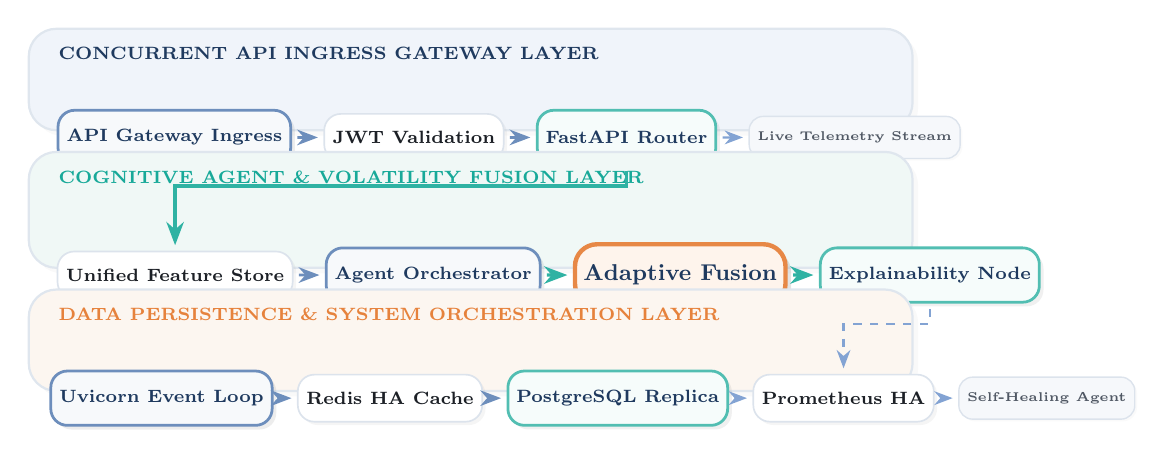
\begin{tikzpicture}[scale=0.92, every node/.style={scale=0.92}, node distance=0.38cm]
  % LAYER 1: API LAYER (Top)
  \node[zoneLayer={bgLayer1}, minimum width=12.2cm, minimum height=1.4cm] (apiZone) {};
  \node[anchor=north west, xshift=0.3cm, yshift=-0.15cm] at (apiZone.north west) {\fontsize{7}{9}\selectfont\bfseries\color{primaryDark} CONCURRENT API INGRESS GATEWAY LAYER};
  
  \node[cardPrimary, xshift=0.4cm, yshift=-0.8cm, anchor=west] (gateway) at (apiZone.west) {API Gateway Ingress};
  \node[cardNode, right=0.4cm of gateway] (validate) {JWT Validation};
  \node[cardTeal, right=0.4cm of validate] (predict) {FastAPI Router};
  \node[cardSecondary, right=0.4cm of predict, minimum width=2.4cm] (telemetry) {Live Telemetry Stream};

  % LAYER 2: INTELLIGENCE LAYER (Middle)
  \node[zoneLayer={bgLayer2}, minimum width=12.2cm, minimum height=1.6cm, below=0.25cm of apiZone] (intelZone) {};
  \node[anchor=north west, xshift=0.3cm, yshift=-0.15cm] at (intelZone.north west) {\fontsize{7}{9}\selectfont\bfseries\color{accentTeal} COGNITIVE AGENT \& VOLATILITY FUSION LAYER};
  
  \node[cardNode, xshift=0.4cm, yshift=-0.9cm, anchor=west] (feat) at (intelZone.west) {Unified Feature Store};
  \node[cardPrimary, right=0.4cm of feat] (orches) {Agent Orchestrator};
  \node[cardHighlight, right=0.4cm of orches] (fusion) {Adaptive Fusion};
  \node[cardTeal, right=0.4cm of fusion] (xai) {Explainability Node};

  % LAYER 3: INFRASTRUCTURE LAYER (Bottom)
  \node[zoneLayer={bgLayer3}, minimum width=12.2cm, minimum height=1.4cm, below=0.25cm of intelZone] (infraZone) {};
  \node[anchor=north west, xshift=0.3cm, yshift=-0.15cm] at (infraZone.north west) {\fontsize{7}{9}\selectfont\bfseries\color{accentOrangeDark} DATA PERSISTENCE \& SYSTEM ORCHESTRATION LAYER};
  
  \node[cardPrimary, xshift=0.3cm, yshift=-0.8cm, anchor=west] (fastapi) at (infraZone.west) {Uvicorn Event Loop};
  \node[cardNode, right=0.3cm of fastapi, minimum width=2.0cm] (redis) {Redis HA Cache};
  \node[cardTeal, right=0.3cm of redis, minimum width=2.0cm] (pgsql) {PostgreSQL Replica};
  \node[cardNode, right=0.3cm of pgsql, minimum width=2.0cm] (prom) {Prometheus HA};
  \node[cardSecondary, right=0.3cm of prom, minimum width=2.0cm] (k8s) {Self-Healing Agent};

  % Arrows & Flow Routing (orthogonal and minimal crossing)
  \draw[flowArrow] (gateway.east) -- (validate.west);
  \draw[flowArrow] (validate.east) -- (predict.west);
  \draw[flowArrowDashed] (predict.east) -- (telemetry.west);
  
  % Vertical bridges
  \draw[flowArrowAccent] (predict.south) -- ++(0,-0.28) -| (feat.north);
  \draw[flowArrow] (feat.east) -- (orches.west);
  \draw[flowArrowAccent] (orches.east) -- (fusion.west);
  \draw[flowArrowAccent] (fusion.east) -- (xai.west);
  
  % Bridges to Infra
  \draw[flowArrowDashed] (xai.south) -- ++(0,-0.28) -| (prom.north);
  
  % Infra flow
  \draw[flowArrow] (fastapi.east) -- (redis.west);
  \draw[flowArrow] (redis.east) -- (pgsql.west);
  \draw[flowArrowDashed] (pgsql.east) -- (prom.west);
  \draw[flowArrowDashed] (prom.east) -- (k8s.west);
\end{tikzpicture}
\vspace{0.05cm}
\centering{\scriptsize\color{textMedium}Integrated multi-layer topology with distinct API, cognitive intelligence, and physical infrastructure zones.}
\end{frame}

% --- SLIDE 7: RUNTIME LIFECYCLE (HERO) ---
\begin{frame}{Runtime Prediction Lifecycle — Async Flow}
\centering
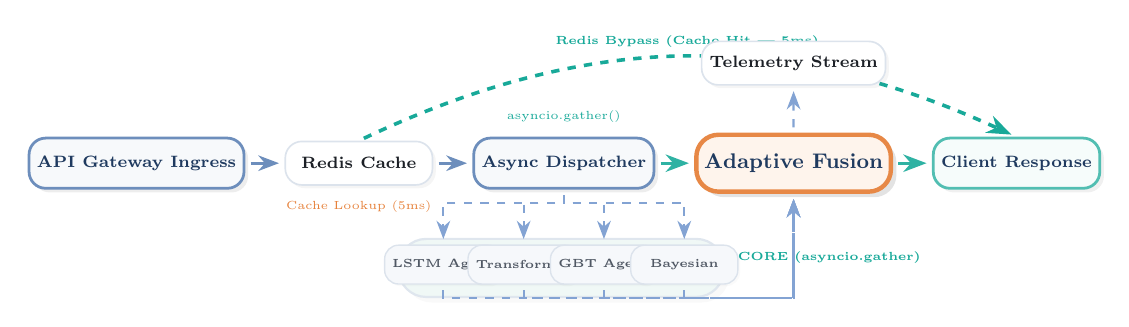
\begin{tikzpicture}[scale=0.85, every node/.style={scale=0.85}, node distance=0.35cm]
  % Top line: request pipeline
  \node[cardPrimary] (ingress) {API Gateway Ingress};
  \node[cardNode, right=0.5cm of ingress] (cache) {Redis Cache};
  \node[cardPrimary, right=0.5cm of cache] (dispatch) {Async Dispatcher};
  \node[cardHighlight, right=0.5cm of dispatch] (fusion) {Adaptive Fusion};
  \node[cardTeal, right=0.5cm of fusion] (response) {Client Response};

  % Redis Short-Circuit Bypass Curve
  \draw[flowArrowDashed, accentTeal, line width=1.3pt, bend left=25] (cache.north) to node[above, font=\tiny\bfseries\color{accentTeal}] {Redis Bypass (Cache Hit — 5ms)} (response.north);

  % Downwards parallel lanes (Agent execution pool)
  \node[cardSecondary, below=0.7cm of dispatch, xshift=-1.8cm, minimum width=1.6cm] (lstm) {LSTM Agent};
  \node[cardSecondary, below=0.7cm of dispatch, xshift=-0.6cm, minimum width=1.6cm] (trans) {Transformer};
  \node[cardSecondary, below=0.7cm of dispatch, xshift=0.6cm, minimum width=1.6cm] (gbt) {GBT Agent};
  \node[cardSecondary, below=0.7cm of dispatch, xshift=1.8cm, minimum width=1.6cm] (bayes) {Bayesian};

  % Grouping the reasoning agents inside a zone!
  \begin{scope}[on background layer]
    \node[zoneLayer={bgLayer2}, fit=(lstm) (bayes), inner sep=0.18cm, yshift=-0.05cm] (agentZone) {};
    \node[anchor=north west, xshift=0.2cm, yshift=-0.08cm] at (agentZone.north west) {\fontsize{5}{6}\selectfont\bfseries\color{accentTeal} CONCURRENT AGENT REASONING CORE (asyncio.gather)};
  \end{scope}

  % Side channel
  \node[cardNode, above=0.6cm of fusion] (tele) {Telemetry Stream};

  % Connect top line
  \draw[flowArrow] (ingress.east) -- (cache.west);
  \draw[flowArrow] (cache.east) -- (dispatch.west);
  \draw[flowArrowAccent] (dispatch.east) -- (fusion.west);
  \draw[flowArrowAccent] (fusion.east) -- (response.west);

  % Connect dispatch to agents (orthogonal routing)
  \draw[flowArrowDashed] (dispatch.south) -- ++(0,-0.2) -| (lstm.north);
  \draw[flowArrowDashed] (dispatch.south) -- ++(0,-0.2) -| (trans.north);
  \draw[flowArrowDashed] (dispatch.south) -- ++(0,-0.2) -| (gbt.north);
  \draw[flowArrowDashed] (dispatch.south) -- ++(0,-0.2) -| (bayes.north);

  % Connect agents to fusion (orthogonal routing)
  \draw[flowArrowDashed] (lstm.south) -- ++(0,-0.2) -| (fusion.south);
  \draw[flowArrowDashed] (trans.south) -- ++(0,-0.2) -| (fusion.south);
  \draw[flowArrowDashed] (gbt.south) -- ++(0,-0.2) -| (fusion.south);
  \draw[flowArrowDashed] (bayes.south) -- ++(0,-0.2) -| (fusion.south);

  % Telemetry channel
  \draw[flowArrowDashed] (fusion.north) -- (tele.south);

  % Custom labels on canvas
  \node[font=\tiny\color{accentOrangeDark}, below=0.08cm of cache] {Cache Lookup (5ms)};
  \node[font=\tiny\color{accentTeal}, above=0.08cm of dispatch] {asyncio.gather()};
\end{tikzpicture}
\vspace{0.05cm}
\begin{columns}[T]
  \column{0.48\textwidth}
  \begin{smallcard}[\linewidth]
    \scriptsize \color{primaryDark}\bfseries 1. Cache-First Logic (Latency Short-Circuit)\\
    \scriptsize \color{textMedium}Redis checks for existing predictions and short-circuits repeat market queries under 5ms, avoiding agent processing entirely.
  \end{smallcard}
  \column{0.48\textwidth}
  \begin{smallcard}[\linewidth]
    \scriptsize \color{accentTeal}\bfseries 2. Parallel Orchestration \& Side-Channel Telemetry\\
    \scriptsize \color{textMedium}Dispatcher schedules multiple agents concurrently using async coroutines. Performance metrics are streamed asynchronously.
  \end{smallcard}
\end{columns}
\end{frame}

% --- SLIDE 8: MULTI-AGENT INTELLIGENCE ---
\begin{frame}{Multi-Agent Intelligence — Forecast Diversity}
\begin{columns}[T]
\column{0.48\textwidth}
\begin{smallcard}[\linewidth]
\centering\bfseries\color{primary}Agent Portfolio
\vspace{0.05cm}
\scriptsize
\begin{itemize}\setlength{\itemsep}{0.2ex}
    \item LSTM: temporal patterns and seasonality
    \item Transformer: attention-based trend context
    \item Gradient Boosted Trees: feature-rich market signals
    \item Bayesian models: uncertainty-aware priors
\end{itemize}
\end{smallcard}
\column{0.48\textwidth}
\begin{smallcard}[\linewidth]
\centering\bfseries\color{accentTeal}Role in the Ensemble
\vspace{0.05cm}
\scriptsize
\begin{itemize}\setlength{\itemsep}{0.2ex}
    \item Diversity reduces correlated failures
    \item Model-specific signals capture different volatility drivers
    \item Output heterogeneity enables conflict-aware fusion
    \item Parallel inference preserves low latency
\end{itemize}
\end{smallcard}
\end{columns}
\end{frame}
% --- SLIDE 9: AGENT COMMUNICATION FLOW ---
% --- SLIDE 9: AGENT COMMUNICATION FLOW ---
\begin{frame}{Agent Communication Flow — Distributed Cognition}
\centering
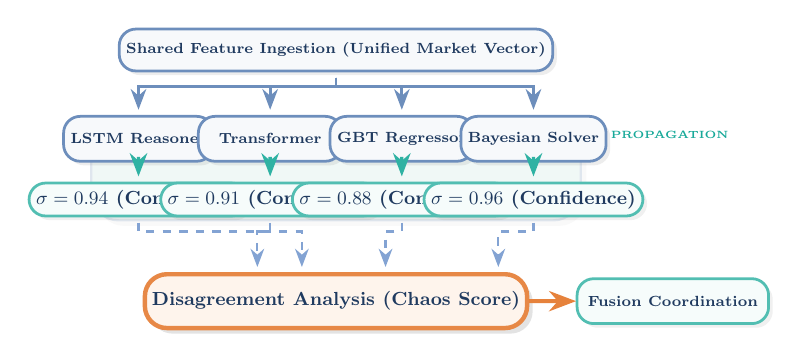
\begin{tikzpicture}[scale=0.74, every node/.style={scale=0.76}, node distance=0.32cm]
  % 1. Shared Feature Ingestion (Top)
  \node[cardPrimary, minimum width=5.5cm, minimum height=0.7cm] (ingest) {Shared Feature Ingestion (Unified Market Vector)};

  % 2. 4 Parallel Lanes for Independent Reasoning
  \node[cardPrimary, below=0.55cm of ingest, xshift=-3.3cm] (lstm) {LSTM Reasoner};
  \node[cardTeal, below=0.25cm of lstm, minimum width=2.0cm, minimum height=0.55cm] (lstm_c) {\small $\sigma = 0.94$ (Confidence)};
  
  \node[cardPrimary, below=0.55cm of ingest, xshift=-1.1cm] (trans) {Transformer};
  \node[cardTeal, below=0.25cm of trans, minimum width=2.0cm, minimum height=0.55cm] (trans_c) {\small $\sigma = 0.91$ (Confidence)};

  \node[cardPrimary, below=0.55cm of ingest, xshift=1.1cm] (gbt) {GBT Regressor};
  \node[cardTeal, below=0.25cm of gbt, minimum width=2.0cm, minimum height=0.55cm] (gbt_c) {\small $\sigma = 0.88$ (Confidence)};

  \node[cardPrimary, below=0.55cm of ingest, xshift=3.3cm] (bayes) {Bayesian Solver};
  \node[cardTeal, below=0.25cm of bayes, minimum width=2.0cm, minimum height=0.55cm] (bayes_c) {\small $\sigma = 0.96$ (Confidence)};

  % Grouping the reasoning agents inside a zone!
  \begin{scope}[on background layer]
    \node[zoneLayer={bgLayer2}, fit=(lstm) (lstm_c) (bayes) (bayes_c), inner sep=0.18cm, yshift=-0.08cm] (reasonZone) {};
    \node[anchor=north west, xshift=0.2cm, yshift=-0.05cm] at (reasonZone.north west) {\fontsize{5}{6}\selectfont\bfseries\color{accentTeal} DECENTRALIZED COGNITIVE AGENT ENGINE \& CONFIDENCE PROPAGATION};
  \end{scope}

  % 3. Bottom Layer: Disagreement & Fusion Coordination
  \node[cardHighlight, below=1.4cm of trans, xshift=1.1cm, minimum width=4.5cm, minimum height=0.9cm] (disagree) {Disagreement Analysis (Chaos Score)};
  \node[cardTeal, right=0.6cm of disagree, minimum width=3.2cm] (fusion) {Fusion Coordination};

  % Ingestion arrows to reasoners
  \draw[flowArrow] (ingest.south) -- ++(0,-0.25) -| (lstm.north);
  \draw[flowArrow] (ingest.south) -- ++(0,-0.25) -| (trans.north);
  \draw[flowArrow] (ingest.south) -- ++(0,-0.25) -| (gbt.north);
  \draw[flowArrow] (ingest.south) -- ++(0,-0.25) -| (bayes.north);

  % Core to Confidence flows (vertical down)
  \draw[flowArrowAccent] (lstm.south) -- (lstm_c.north);
  \draw[flowArrowAccent] (trans.south) -- (trans_c.north);
  \draw[flowArrowAccent] (gbt.south) -- (gbt_c.north);
  \draw[flowArrowAccent] (bayes.south) -- (bayes_c.north);

  % Routing from Confidence outputs to Disagreement Engine and Fusion Coordination
  \draw[flowArrowDashed] (lstm_c.south) -- ++(0,-0.25) -| (disagree.140);
  \draw[flowArrowDashed] (trans_c.south) -- ++(0,-0.25) -| (disagree.160);
  \draw[flowArrowDashed] (gbt_c.south) -- ++(0,-0.25) -| (disagree.30);
  \draw[flowArrowDashed] (bayes_c.south) -- ++(0,-0.25) -| (disagree.10);

  % Link Disagreement engine to Fusion Coordination
  \draw[->, >=Stealth, line width=1.5pt, accentOrangeDark] (disagree.east) -- (fusion.west);
\end{tikzpicture}
\vspace{0.05cm}
\begin{columns}[T]
  \column{0.48\textwidth}
  \begin{smallcard}[\linewidth]
    \scriptsize \color{primaryDark}\bfseries 1. Shared Ingestion \& Independent Reasoning\\
    \scriptsize \color{textMedium}A unified feature vector is dispatched concurrently to diverse agents. Each agent reasons independently, outputting a raw forecast and local confidence score.
  \end{smallcard}
  \column{0.48\textwidth}
  \begin{smallcard}[\linewidth]
    \scriptsize \color{accentTeal}\bfseries 2. Conflict Analysis \& Fusion Coordination\\
    \scriptsize \color{textMedium}Confidence scores are propagated to the Disagreement Engine, which computes conflict dynamics and modulates fusion weights before output.
  \end{smallcard}
\end{columns}
\end{frame}

% --- SLIDE 10: EXPLAINABILITY LAYER ---
\begin{frame}{Explainability Layer — Decision Transparency}
\begin{herocard}
\begin{columns}[T]
\column{0.56\textwidth}
\begin{itemize}
    \scriptsize
    \item SHAP at inference: feature contributions per forecast
    \item Counterfactual scenarios for "what-if" market outcomes
    \item Confidence streaming: reliability score for each ensemble decision
    \item Domain metadata attaches crop, mandi, and policy context
\end{itemize}
\column{0.44\textwidth}
\begin{smallcard}
\centering\bfseries\color{accentOrange}Explainability Outputs
\vspace{0.1cm}
\scriptsize
\begin{itemize}
    \item Top drivers of each price prediction
    \item Volatility alerts with root cause signals
    \item Actionable advisory explanations for traders
\end{itemize}
\end{smallcard}
\end{columns}
\end{herocard}
\end{frame}

% --- SLIDE 11: ASK-YOUR-DATA INTELLIGENCE ---
\begin{frame}{Ask-Your-Data Intelligence}
\begin{herocard}
\begin{itemize}
    \scriptsize
    \item Integrated question-driven analysis for traders, analysts, and cooperatives
    \item Natural language query interface over mandi, crop, and market signal datasets
    \item Produces forecast summaries, risk score narratives, and decision prompts
    \item Accelerates domain exploration during shock events and regime shifts
\end{itemize}
\end{herocard}
\end{frame}

% --- SLIDE 12: ONLINE VS OFFLINE PIPELINE ---
\begin{frame}{Online vs Offline ML Pipeline}
\begin{columns}[T]
\column{0.48\textwidth}
\begin{smallcard}[\linewidth]
\centering\bfseries\color{primary}Offline Training
\vspace{0.05cm}
\scriptsize
\begin{itemize}\setlength{\itemsep}{0.2ex}
    \item Historical model training on segmented mandi datasets
    \item Feature engineering using weather, logistics, and market signals
    \item Periodic model retraining and backtest validation
    \item Batch evaluation of volatility regime handlers
\end{itemize}
\end{smallcard}
\column{0.48\textwidth}
\begin{smallcard}[\linewidth]
\centering\bfseries\color{accentEmerald}Online Inference
\vspace{0.05cm}
\scriptsize
\begin{itemize}\setlength{\itemsep}{0.2ex}
    \item Low-latency request handling via FastAPI
    \item Redis caching of stable forecasts and intermediate state
    \item Parallel agent execution with asyncio
    \item Continuous telemetry and explainability logging
\end{itemize}
\end{smallcard}
\end{columns}
\end{frame}

% --- SLIDE 8: META-ENSEMBLE (HERO — CORE RESEARCH) ---
\begin{frame}{Adaptive Meta-Ensemble — The Intelligence Core}
\centering
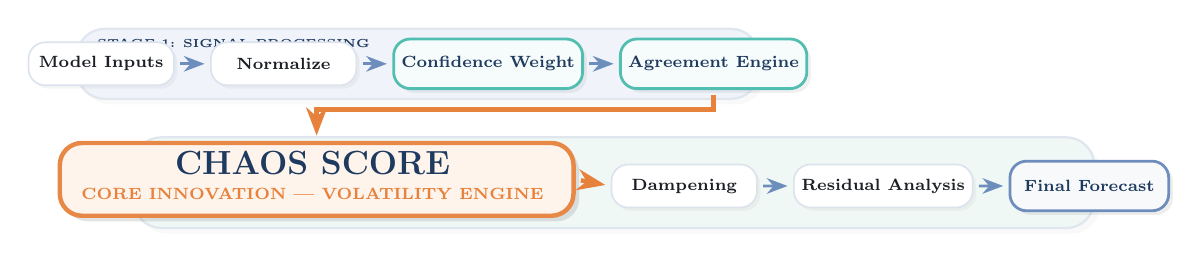
\begin{tikzpicture}[scale=0.84, every node/.style={scale=0.84}, node distance=0.35cm]
  % ROW 1: PREPARATION & EVALUATION
  \node[cardNode] (input) {Model Inputs};
  \node[cardNode, right=0.45cm of input] (norm) {Normalize};
  \node[cardTeal, right=0.45cm of norm] (weight) {Confidence Weight};
  \node[cardTeal, right=0.45cm of weight] (agree) {Agreement Engine};
  
  % ROW 2: FUSION & OUTLIER CONTROL
  % Chaos Score dominates: positioned below Col 1 and 2
  \node[cardHighlight, below=0.7cm of norm, xshift=0.5cm, minimum width=4.8cm, minimum height=1.1cm] (chaos) {
    \begin{tabular}{c}
      \bfseries\Large CHAOS SCORE \\
      \fontsize{7}{8}\selectfont\color{accentOrangeDark}\bfseries CORE INNOVATION — VOLATILITY ENGINE
    \end{tabular}
  };
  
  \node[cardNode, right=0.45cm of chaos, yshift=-0.1cm] (damp) {Dampening};
  \node[cardNode, right=0.45cm of damp] (res) {Residual Analysis};
  \node[cardPrimary, right=0.45cm of res] (final) {Final Forecast};
  
  % Connection routing
  \draw[flowArrow] (input.east) -- (norm.west);
  \draw[flowArrow] (norm.east) -- (weight.west);
  \draw[flowArrow] (weight.east) -- (agree.west);
  
  % Connect Row 1 to Row 2
  \draw[->, >=Stealth, line width=1.6pt, accentOrangeDark, shorten >=2pt, shorten <=2pt] (agree.south) -- ++(0,-0.3) -| (chaos.north);
  
  % Row 2 flow
  \draw[->, >=Stealth, line width=1.6pt, accentOrangeDark, shorten >=2pt, shorten <=2pt] (chaos.east) -- (damp.west);
  \draw[flowArrow] (damp.east) -- (res.west);
  \draw[flowArrow] (res.east) -- (final.west);
  
  % Subtle background box grouping for Row 1
  \begin{scope}[on background layer]
    \node[zoneLayer={bgLayer1}, fit=(input) (norm) (weight) (agree), inner sep=0.2cm] (row1Zone) {};
    \node[anchor=north west, xshift=0.2cm, yshift=-0.05cm] at (row1Zone.north west) {\tiny\bfseries\color{primaryDark} STAGE 1: SIGNAL PROCESSING};
    
    \node[zoneLayer={bgLayer2}, fit=(chaos) (damp) (res) (final), inner sep=0.2cm, yshift=-0.05cm] (row2Zone) {};
    \node[anchor=north west, xshift=0.2cm, yshift=-0.05cm] at (row2Zone.north west) {\tiny\bfseries\color{accentTeal} STAGE 2: VOLATILITY ADAPTIVE FUSION};
  \end{scope}
\end{tikzpicture}
\vspace{0.05cm}
\begin{columns}[T]
  \column{0.48\textwidth}
  \begin{smallcard}[\linewidth]
    \scriptsize \color{primaryDark}\bfseries Phase 1: Normalization \& Multi-Agent Weighting\\
    \scriptsize \color{textMedium}Ensures predictions from heterogeneous agents (LSTM, GBT, Bayesian) are scaled properly and weighted based on rolling historical accuracy.
  \end{smallcard}
  \column{0.48\textwidth}
  \begin{smallcard}[\linewidth]
    \scriptsize \color{accentOrangeDark}\bfseries Phase 2: Dynamic Chaos Scoring \& Outlier Shield\\
    \scriptsize \color{textMedium}The \textbf{Chaos Score} detects disagreement and scales down weights in high-volatility regimes. Dampening \& Residual filters shield against outliers.
  \end{smallcard}
\end{columns}
\end{frame}

% --- SLIDE 9: VOLATILITY ---
\begin{frame}{Volatility \& Regime Intelligence}
\begin{columns}[T]
\column{0.48\textwidth}
\begin{smallcard}[\linewidth]
\centering\bfseries\color{primary}\large Volatility Detection Engine
\vspace{0.05cm}
\begin{itemize}\setlength{\itemsep}{0.2ex}\setlength{\parskip}{0pt}
    \footnotesize
    \item \textbf{GARCH}: Conditional volatility
    \item \textbf{HMM}: Regime estimation
    \item \textbf{2$\sigma$ Alerts}: Anomaly detection
\end{itemize}
\end{smallcard}
\column{0.48\textwidth}
\begin{smallcard}[\linewidth]
\centering\bfseries\color{accentTeal}\large Adaptive Response
\vspace{0.05cm}
\begin{itemize}\setlength{\itemsep}{0.2ex}\setlength{\parskip}{0pt}
    \footnotesize
    \item Low $\rightarrow$ Standard weights
    \item High $\rightarrow$ Conservative fusion
    \item Crisis $\rightarrow$ Max penalty
\end{itemize}
\end{smallcard}
\end{columns}
\vspace{0.05cm}
\centering{\small\color{textMedium}Regime change triggers adaptive ensemble behavior in real-time}
\end{frame}

% ============================================================
% SECTION 03: INFRASTRUCTURE ENGINEERING
% ============================================================
\sectiontransition{03}{Infrastructure Engineering}{Building Operationally Resilient AI Systems}

% --- SLIDE 10: ASYNC BACKEND (HERO) ---
\begin{frame}{Async Backend — Parallel Market Reasoning}
\centering
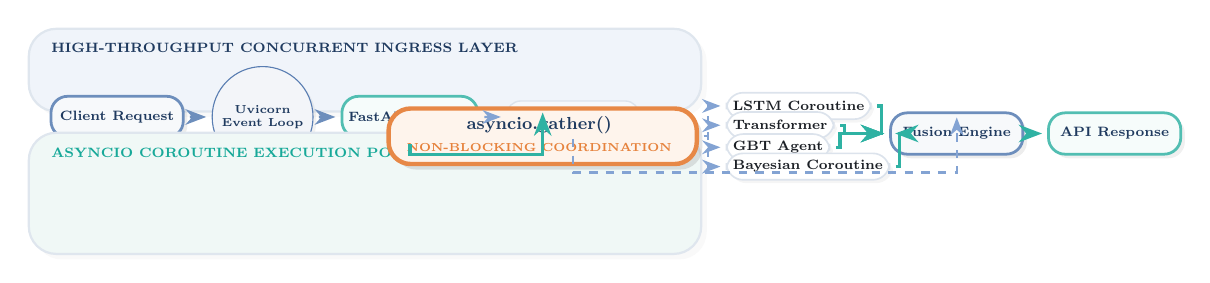
\begin{tikzpicture}[scale=0.62, every node/.style={scale=0.70}, node distance=0.35cm]
  % Grouped background zones for process steps
  \node[zoneLayer={bgLayer1}, minimum width=12.2cm, minimum height=1.5cm] (apiZone) {};
  \node[anchor=north west, xshift=0.3cm, yshift=-0.15cm] at (apiZone.north west) {\fontsize{7}{9}\selectfont\bfseries\color{primaryDark} HIGH-THROUGHPUT CONCURRENT INGRESS LAYER};
  
  \node[cardPrimary, xshift=0.4cm, yshift=-0.85cm, anchor=west] (client) at (apiZone.west) {Client Request};
  % Event Loop styled as an elegant spinning circle!
  \node[circle, draw=primary!80, fill=primary!6, minimum size=1.3cm, align=center, font=\fontsize{6}{7}\selectfont\bfseries\color{primaryDark}, drop shadow={shadow xshift=1.2pt, shadow yshift=-1.2pt, opacity=0.1}, right=0.35cm of client] (uvicorn) {Uvicorn\\Event Loop};
  \node[cardTeal, right=0.35cm of uvicorn] (router) {FastAPI Router};
  \node[cardSecondary, right=0.35cm of router, minimum width=2.4cm] (bgTask) {BackgroundTasks};

  \node[zoneLayer={bgLayer2}, minimum width=12.2cm, minimum height=2.2cm, below=0.25cm of apiZone] (engineZone) {};
  \node[anchor=north west, xshift=0.3cm, yshift=-0.15cm] at (engineZone.north west) {\fontsize{7}{9}\selectfont\bfseries\color{accentTeal} ASYNCIO COROUTINE EXECUTION POOL (NON-BLOCKING WORKERS)};
  
  \node[cardHighlight, xshift=0.4cm, yshift=-1.2cm, anchor=west, minimum width=3.4cm] (gather) {
    \begin{tabular}{c}
      \bfseries asyncio.gather() \\
      \fontsize{6}{7}\selectfont\color{accentOrangeDark}\bfseries NON-BLOCKING COORDINATION
    \end{tabular}
  };
  
  \node[cardNode, right=0.35cm of gather, yshift=0.55cm, minimum width=1.8cm, minimum height=0.48cm] (a1) {LSTM Coroutine};
  \node[cardNode, right=0.35cm of gather, yshift=0.2cm, minimum width=1.8cm, minimum height=0.48cm] (a2) {Transformer};
  \node[cardNode, right=0.35cm of gather, yshift=-0.2cm, minimum width=1.8cm, minimum height=0.48cm] (a3) {GBT Agent};
  \node[cardNode, right=0.35cm of gather, yshift=-0.55cm, minimum width=1.8cm, minimum height=0.48cm] (a4) {Bayesian Coroutine};
  
  \node[cardPrimary, right=0.35cm of a2, xshift=0.5cm, yshift=-0.15cm] (fusion) {Fusion Engine};
  \node[cardTeal, right=0.3cm of fusion] (response) {API Response};

  % Routing arrows
  \draw[flowArrow] (client.east) -- (uvicorn.west);
  \draw[flowArrow] (uvicorn.east) -- (router.west);
  \draw[flowArrowDashed] (router.east) -- (bgTask.west);
  
  % Connection to asyncio.gather
  \draw[flowArrowAccent] (router.south) -- ++(0,-0.32) -| (gather.north);
  
  % Connect gather to agents
  \draw[flowArrowDashed] (gather.east) -- ++(0.2,0) |- (a1.west);
  \draw[flowArrowDashed] (gather.east) -- ++(0.2,0) |- (a2.west);
  \draw[flowArrowDashed] (gather.east) -- ++(0.2,0) |- (a3.west);
  \draw[flowArrowDashed] (gather.east) -- ++(0.2,0) |- (a4.west);
  
  % Connect agents to fusion
  \draw[flowArrowAccent] (a1.east) -- ++(0.2,0) |- (fusion.west);
  \draw[flowArrowAccent] (a2.east) -- ++(0.2,0) |- (fusion.west);
  \draw[flowArrowAccent] (a3.east) -- ++(0.2,0) |- (fusion.west);
  \draw[flowArrowAccent] (a4.east) -- ++(0.2,0) |- (fusion.west);
  
  % Connect fusion to response
  \draw[flowArrowAccent] (fusion.east) -- (response.west);
  
  % Non-blocking side channel
  \draw[flowArrowDashed] (bgTask.south) -- ++(0,-0.8) -| (fusion.north);
\end{tikzpicture}
\vspace{0.05cm}
\begin{columns}[T]
  \column{0.48\textwidth}
  \begin{smallcard}[\linewidth]
    \scriptsize \color{primaryDark}\bfseries 1. Non-Blocking Event Loop (Uvicorn/FastAPI)\\
    \scriptsize \color{textMedium}Leverages `uvloop` for high-throughput HTTP handling. Incoming requests spawn concurrent task threads that yield execution while awaiting I/O.
  \end{smallcard}
  \column{0.48\textwidth}
  \begin{smallcard}[\linewidth]
    \scriptsize \color{accentTeal}\bfseries 2. Orchestrated asyncio.gather() Execution\\
    \scriptsize \color{textMedium}Forecast agents run concurrently inside the coroutine loop. Disagreement scoring and fusion occur in-memory, ensuring sub-15ms overhead.
  \end{smallcard}
\end{columns}
\end{frame}

% --- SLIDE 11: DEPLOYMENT TOPOLOGY (HERO) ---
\begin{frame}{Deployment Topology — Production Infrastructure}
\centering
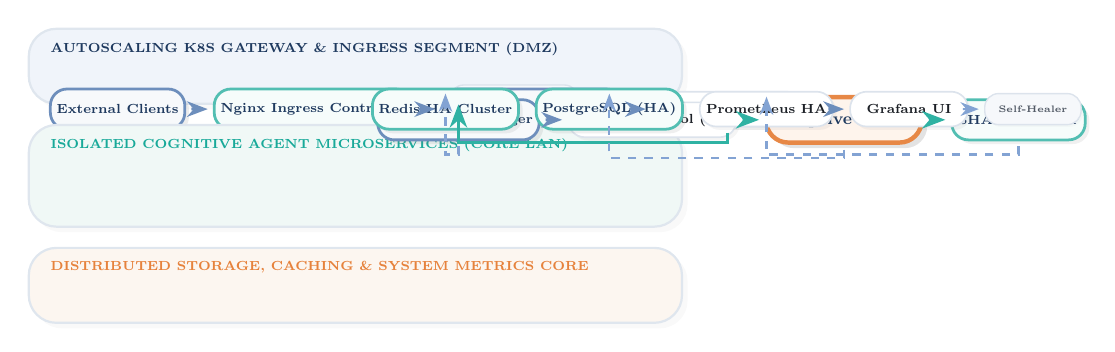
\begin{tikzpicture}[scale=0.62, every node/.style={scale=0.68}, node distance=0.32cm]
  % 1. Ingress Layer
  \node[zoneLayer={bgLayer1}, minimum width=12.2cm, minimum height=1.4cm] (ingressZone) {};
  \node[anchor=north west, xshift=0.3cm, yshift=-0.15cm] at (ingressZone.north west) {\fontsize{7}{9}\selectfont\bfseries\color{primaryDark} AUTOSCALING K8S GATEWAY \& INGRESS SEGMENT (DMZ)};
  
  \node[cardPrimary, xshift=0.4cm, yshift=-0.8cm, anchor=west] (clients) at (ingressZone.west) {External Clients};
  \node[cardTeal, right=0.35cm of clients] (ingress) {Nginx Ingress Controller};
  
  % Triple-stacked replica gateway pods for visual K8s realistic replication!
  \node[cardSecondary, right=0.35cm of ingress, xshift=0.16cm, yshift=0.16cm, minimum width=2.4cm] (gw_stack3) {};
  \node[cardSecondary, right=0.35cm of ingress, xshift=0.08cm, yshift=0.08cm, minimum width=2.4cm] (gw_stack2) {Gateway Pod (Replica)};
  \node[cardPrimary, right=0.35cm of ingress, minimum width=2.4cm] (gateway) {FastAPI Gateway (x3)};
  \node[cardNode, right=0.35cm of gateway] (auth) {JWT Auth Engine};

  % 2. Core Service Layer
  \node[zoneLayer={bgLayer2}, minimum width=12.2cm, minimum height=1.9cm, below=0.25cm of ingressZone] (coreZone) {};
  \node[anchor=north west, xshift=0.3cm, yshift=-0.15cm] at (coreZone.north west) {\fontsize{7}{9}\selectfont\bfseries\color{accentTeal} ISOLATED COGNITIVE AGENT MICROSERVICES (CORE LAN)};
  
  \node[cardPrimary, xshift=0.4cm, yshift=-1.0cm, anchor=west] (orches) {Prediction Manager};
  \node[cardNode, right=0.35cm of orches] (agents) {Agent Pod Pool (x4)};
  \node[cardHighlight, right=0.35cm of agents] (fusion) {Adaptive Fusion};
  \node[cardTeal, right=0.35cm of fusion] (xai) {SHAP Streamer};

  % 3. Infrastructure & Observability Layer
  \node[zoneLayer={bgLayer3}, minimum width=12.2cm, minimum height=1.4cm, below=0.25cm of coreZone] (infraZone) {};
  \node[anchor=north west, xshift=0.3cm, yshift=-0.15cm] at (infraZone.north west) {\fontsize{7}{9}\selectfont\bfseries\color{accentOrangeDark} DISTRIBUTED STORAGE, CACHING \& SYSTEM METRICS CORE};
  
  \node[cardTeal, xshift=0.3cm, yshift=-0.8cm, anchor=west, minimum width=2.2cm] (redis) {Redis HA Cluster};
  \node[cardTeal, right=0.2cm of redis, minimum width=2.2cm] (pgsql) {PostgreSQL (HA)};
  \node[cardNode, right=0.2cm of pgsql, minimum width=2.2cm] (prom) {Prometheus HA};
  \node[cardNode, right=0.2cm of prom, minimum width=2.2cm] (graf) {Grafana UI};
  \node[cardSecondary, right=0.2cm of graf, minimum width=1.8cm] (k8s) {Self-Healer};

  % Connecting lines
  \draw[flowArrow] (clients.east) -- (ingress.west);
  \draw[flowArrow] (ingress.east) -- (gateway.west);
  \draw[flowArrow] (gateway.east) -- (auth.west);
  
  % Ingress to Core
  \draw[flowArrowAccent] (auth.south) -- ++(0,-0.32) -| (orches.north);
  
  % Core horizontal flows
  \draw[flowArrow] (orches.east) -- (agents.west);
  \draw[flowArrowAccent] (agents.east) -- (fusion.west);
  \draw[flowArrowAccent] (fusion.east) -- (xai.west);
  
  % Core to Storage (vertical paths)
  \draw[flowArrowDashed] (orches.south) -- ++(0,-0.28) -| (redis.north);
  \draw[flowArrowDashed] (fusion.south) -- ++(0,-0.28) -| (pgsql.north);
  \draw[flowArrowDashed] (xai.south) -- ++(0,-0.28) -| (prom.north);
  
  % Infra monitoring flows
  \draw[flowArrow] (prom.east) -- (graf.west);
  \draw[flowArrowDashed] (graf.east) -- (k8s.west);
\end{tikzpicture}
\vspace{0.05cm}
\begin{columns}[T]
  \column{0.48\textwidth}
  \begin{smallcard}[\linewidth]
    \scriptsize \color{primaryDark}\bfseries 1. Autoscaling Gateway \& Cognitive Core\\
    \scriptsize \color{textMedium}Gateways scale dynamically under burst load. Core services reside in isolated namespaces, routing queries to dedicated model containers.
  \end{smallcard}
  \column{0.48\textwidth}
  \begin{smallcard}[\linewidth]
    \scriptsize \color{accentOrangeDark}\bfseries 2. Active Storage \& Self-Healing Loop\\
    \scriptsize \color{textMedium}High-availability Redis coordinates caching, while Prometheus feeds the custom Self-Healer operator to auto-restart degraded components.
  \end{smallcard}
\end{columns}
\end{frame}

% --- SLIDE 11A: FASTAPI RUNTIME ---
\begin{frame}{FastAPI Runtime — Production Service}
\begin{herocard}
\begin{itemize}
    \small
    \item REST and WebSocket endpoints unify forecasting, monitoring, and explainability services
    \item Async request handling preserves sub-200ms p95 latency under concurrent load
    \item Rate limiting and validation protect against malformed market requests
    \item Health checks, startup probes, and graceful shutdown enable production readiness
\end{itemize}
\end{herocard}
\end{frame}

% --- SLIDE 11B: REDIS CACHING SYSTEM ---
\begin{frame}{Redis Caching System}
\begin{herocard}
\begin{itemize}
    \small
    \item Short-circuits repeated lookups for stable market forecasts
    \item Stores input features, prediction cache, and stateful agent metadata
    \item Fine-grained TTLs support market freshness and volatility invalidation
    \item Supports burst load smoothing and fast retrieval for repeat requests
\end{itemize}
\end{herocard}
\end{frame}

% --- SLIDE 11C: POSTGRESQL PERSISTENCE ---
\begin{frame}{PostgreSQL Persistence — Historical Intelligence}
\begin{herocard}
\begin{itemize}
    \small
    \item Stores feature snapshots, forecast records, event logs, and explainability traces
    \item Enables auditability, retrospective analysis, and regulatory reporting
    \item Indexes on mandi, crop, timestamp, and regime labels for fast queries
    \item Supports batch ingestion and long-term model evaluation storage
\end{itemize}
\end{herocard}
\end{frame}

% --- SLIDE 11D: MONITORING & TELEMETRY ---
\begin{frame}{Monitoring \& Telemetry — Observability Stack}
\begin{herocard}
\begin{itemize}
    \small
    \item Captures request latency, cache hits, agent response times, and error rates
    \item Produces distributed traces for API, orchestration, and model execution
    \item Stores telemetry in time-series engine for alerting and trend analysis
    \item Enables root-cause diagnostics for pipeline slowdowns and volatility anomalies
\end{itemize}
\end{herocard}
\end{frame}

% --- SLIDE 11E: PROMETHEUS METRICS ---
\begin{frame}{Prometheus Metrics — Live Performance Signals}
\begin{herocard}
\begin{itemize}
    \small
    \item Tracks p50/p90/p95 latency, throughput, cache efficiency, and queue depth
    \item Exposes custom metrics for ensemble disagreement, chaos score, and regime transitions
    \item Supports alerting on performance degradation, increased variance, and backend error spikes
    \item Integrates with Grafana dashboards for operational visibility
\end{itemize}
\end{herocard}
\end{frame}

% --- SLIDE 11F: RESILIENCE & CIRCUIT BREAKERS ---
\begin{frame}{Resilience \& Circuit Breakers}
\begin{herocard}
\begin{itemize}
    \small
    \item Circuit breaker patterns isolate failing agents and preserve end-to-end availability
    \item Fallback forecasts and confidence reduction maintain safe outputs when an agent is degraded
    \item Retry policies with exponential backoff protect dependent services
    \item Health probes and auto-recovery logic support operational robustness
\end{itemize}
\end{herocard}
\end{frame}

% --- SLIDE 11G: TRADEROS COGNITION STREAMING ---
\begin{frame}{TraderOS Cognition Streaming}
\begin{herocard}
\begin{itemize}
    \small
    \item Streaming event bus carries market signals, prediction state, and explainability metadata
    \item Enables real-time cognition updates and rule-based action triggers
    \item Supports downstream consumers such as advisory dashboards and institutional risk engines
    \item Provides a coherent stream for continuous learning and operational decisioning
\end{itemize}
\end{herocard}
\end{frame}

% ============================================================
% SECTION 04: EXPERIMENTAL VALIDATION
% ============================================================
\sectiontransition{04}{Experimental Validation}{Validating Forecasting Robustness and Infrastructure Reliability}

% --- SLIDE 12A: EVALUATION METHODOLOGY ---
\begin{frame}{Evaluation Methodology}
\begin{herocard}
\begin{itemize}
    \small
    \item Multi-market evaluation across mandis, crop classes, and time horizons
    \item Baseline comparison against ARIMA, LSTM, Transformer, and static ensemble models
    \item Metrics include RMSE, MAE, volatility stabilization, and regime-aware error
    \item Validation on historical episodes, event shocks, and live replay datasets
\end{itemize}
\end{herocard}
\end{frame}

% --- SLIDE 12B: CHRONOLOGICAL VALIDATION ---
\begin{frame}{Chronological Validation — Staged Confidence}
\begin{columns}[T]
\column{0.48\textwidth}
\begin{smallcard}[\linewidth]
\centering\bfseries\color{primary}Phase 1: Historical Backtest
\vspace{0.05cm}
\scriptsize
\begin{itemize}\setlength{\itemsep}{0.2ex}
    \item Calendarized mandi snapshots
    \item Regime-labelled volatility events
    \item Backtest against known shock windows
\end{itemize}
\end{smallcard}
\column{0.48\textwidth}
\begin{smallcard}[\linewidth]
\centering\bfseries\color{accentTeal}Phase 2: Live Replay
\vspace{0.05cm}
\scriptsize
\begin{itemize}\setlength{\itemsep}{0.2ex}
    \item Replayed real market streams at production cadence
    \item Measured latency, stability, and cache behavior
    \item Verified explainability outputs under market stress
\end{itemize}
\end{smallcard}
\end{columns}
\end{frame}

% --- SLIDE 12C: PREDICTION RELIABILITY ---
\begin{frame}{Prediction Reliability — Confidence \& Regimes}
\begin{herocard}
\begin{itemize}
    \small
    \item Confidence scores quantify the ensemble's forecast reliability
    \item Regime-aware logic reduces risk by penalizing high-disagreement predictions
    \item Reliability banding supports safe decision thresholds for investors and cooperatives
    \item Observed low-confidence alerts reduce blind deployment risk during volatility spikes
\end{itemize}
\end{herocard}
\end{frame}

% --- SLIDE 12D: RESIDUAL ANALYSIS ---
\begin{frame}{Residual Analysis — Forecast Error Diagnostics}
\begin{herocard}
\begin{itemize}
    \small
    \item Residual distributions analyzed for heteroscedasticity and outlier bias
    \item Adaptive dampening reduces extreme residuals from conflicting agents
    \item Post-hoc diagnostic reports identify scenario-specific error drivers
    \item Enables targeted model improvements for low-volume and shock windows
\end{itemize}
\end{herocard}
\end{frame}

% --- SLIDE 12E: INFRASTRUCTURE VALIDATION ---
\begin{frame}{Infrastructure Validation — Operational Reliability}
\begin{herocard}
\begin{itemize}
    \small
    \item Load test validation of FastAPI concurrency and Redis caching
    \item Failover simulation for agent degradation and database recovery
    \item End-to-end trace verification for telemetry and Prometheus alerting
    \item Stability assessment under batch replay and streaming update loads
\end{itemize}
\end{herocard}
\end{frame}

% --- SLIDE 12F: OBJECTIVE FULFILLMENT MAPPING ---
\begin{frame}{Objective Fulfillment Mapping}
\begin{herocard}
\centering
\scriptsize
\begin{tabular}{p{3.2cm}|p{3.4cm}|p{3.4cm}}
\toprule
\bfseries Objective & \bfseries Success Criteria & \bfseries Evidence \\
\midrule
Multi-Agent Forecasting & Diverse agent performance & MandiSense outperforms single-model baselines \\
Volatility-Aware Fusion & Regime-sensitive error reduction & Chaos score reduces high-volatility loss \\
Explainable Decisions & Runtime feature transparency & Integrated SHAP + counterfactual reports \\
Production Infrastructure & Sub-200ms latency & FastAPI + Redis throughput validated \\
\bottomrule
\end{tabular}
\end{herocard}
\end{frame}

% --- SLIDE 12: BENCHMARK (HERO) ---
\begin{frame}{Benchmark Results — Forecasting Accuracy}
\begin{herocard}[0.98\textwidth]
\begin{columns}[T]
  \column{0.56\textwidth}
  \centering
  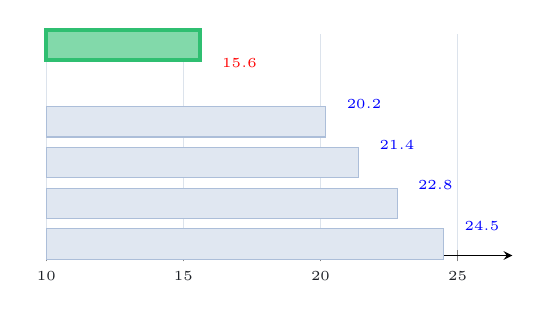
\begin{tikzpicture}
  \begin{axis}[
      xbar,
      width=7.5cm, height=4.4cm,
      xmin=10, xmax=27,
      axis x line=bottom,
      axis y line=none,
      enlarge y limits=0.18,
      ytick=data,
      yticklabels={ARIMA Baseline, LSTM, Transformer, Static Ensemble, \textbf{MandiSense AI}},
      tick label style={font=\tiny, color=textDark},
      nodes near coords,
      nodes near coords align=horizontal,
      bar width=11pt,
      every node near coord/.style={font=\tiny\bfseries, anchor=west, xshift=4pt},
      xmajorgrids=true,
      grid style={draw=borderLight, thin},
      clip=false
  ]
  \addplot+[draw=primary!40, fill=primary!15] coordinates {(24.5,0) (22.8,1) (21.4,2) (20.2,3)};
  \addplot+[draw=accentEmerald, fill=accentEmerald!60, line width=1.5pt] coordinates {(15.6,4)};
  \end{axis}
  \end{tikzpicture}
  
  \column{0.40\textwidth}
  \vspace{0.15cm}
  \begin{mdframed}[
    linewidth=1.2pt,
    linecolor=accentEmerald,
    backgroundcolor=accentEmerald!6,
    roundcorner=6pt,
    innertopmargin=8pt,
    innerbottommargin=8pt,
    innerleftmargin=10pt,
    innerrightmargin=10pt
  ]
    \centering
    {\fontsize{24}{28}\selectfont\bfseries\color{accentEmerald} -22.7\%}\\[0.1cm]
    {\scriptsize\bfseries\color{primaryDark} RMSE ERROR REDUCTION}\\[0.2cm]
    \tiny\color{textMedium} Outperforms all statistical baselines, recurrent neural architectures, and static ensemble fusion platforms.
  \end{mdframed}
  
  \vspace{0.15cm}
  
  \begin{smallcard}[0.98\textwidth]
    \tiny\bfseries\color{primaryDark} Key Research Takeaway\\[0.05cm]
    \tiny\color{textMedium} Static ensemble models degrade under volatility spikes. MandiSense AI maintains high stability by gating agent contributions via the Chaos Score.
  \end{smallcard}
\end{columns}
\end{herocard}
\end{frame}

% --- SLIDE 13: LATENCY ---
\begin{frame}{Operational Validation — Real-Time Performance}
\begin{columns}[T]
\column{0.48\textwidth}
\begin{smallcard}[\linewidth]
\centering\bfseries\color{primary}\large Latency Metrics
\vspace{0.05cm}
\centering
\begin{tabular}{l|c}
\toprule
\bfseries\small Percentile & \bfseries\small Latency \\
\midrule
\scriptsize p50 (median) & \scriptsize 45 ms \\
\scriptsize p90 & \scriptsize 120 ms \\
\color{accentEmerald}\bfseries\scriptsize p95 & \color{accentEmerald}\bfseries\scriptsize 185 ms \\
\scriptsize p99 & \scriptsize 240 ms \\
\bottomrule
\end{tabular}
\end{smallcard}
\column{0.48\textwidth}
\begin{smallcard}[\linewidth]
\centering\bfseries\color{accentTeal}\large Throughput
\vspace{0.05cm}
\centering\normalsize\bfseries 500+ req/s
\vspace{0.1cm}
\centering\fcolorbox{accentEmerald}{accentEmerald!12}{\parbox{2.7cm}{\centering
\scriptsize Target <200ms p95\\ \scriptsize Achieved 185ms}}
\end{smallcard}
\end{columns}
\vspace{0.05cm}
\centering{\small\color{textMedium}Production-ready latency for real-time operational intelligence}
\end{frame}

% --- SLIDE 14: FINDINGS ---
\begin{frame}{Key Findings \& Practical Significance}
\begin{columns}[T]
\column{0.48\textwidth}
\begin{smallcard}[\linewidth]
\centering\bfseries\color{primary}\large Research Insights
\vspace{0.05cm}
\begin{itemize}\setlength{\itemsep}{0.2ex}
    \scriptsize
    \item \textbf{Volatility stabilization}: 41\% variance reduction
    \item \textbf{Conflict as signal}: $\rho=0.73$ with error
    \item \textbf{Grounded XAI}: 84\% domain alignment
\end{itemize}
\end{smallcard}
\column{0.48\textwidth}
\begin{smallcard}[\linewidth]
\centering\bfseries\color{accentOrange}\large Practical Impact
\vspace{0.05cm}
\begin{itemize}\setlength{\itemsep}{0.2ex}
    \scriptsize
    \item \textbf{Farmers}: Actionable 3-day outlook
    \item \textbf{Cooperatives}: Timing optimization
    \item \textbf{Estimated}: 12-18\% loss reduction
\end{itemize}
\end{smallcard}
\end{columns}
\vspace{0.05cm}
\centering{\small\color{textMedium}Evolved forecasting from prediction into operational agricultural decision intelligence}
\end{frame}

% ============================================================
% SECTION 05: FUTURE & CONCLUSION
% ============================================================
\sectiontransition{05}{Future \& Vision}{From Forecasting to Autonomous Agricultural Intelligence}

% --- SLIDE 15: LIMITATIONS & FUTURE ---
\begin{frame}{Limitations \& Future Research Directions}
\begin{columns}[T]
\column{0.48\textwidth}
\begin{smallcard}[\linewidth]
\centering\bfseries\color{primaryDark}\large Current Limitations
\vspace{0.05cm}
\begin{itemize}\setlength{\itemsep}{0.2ex}
    \scriptsize
    \item Data sparsity in low-volume markets
    \item Exogenous shocks (weather, policy)
    \item Daily batch retraining latency
    \item GARCH normality assumptions
\end{itemize}
\end{smallcard}
\column{0.48\textwidth}
\begin{smallcard}[\linewidth]
\centering\bfseries\color{accentTeal}\large Future Intelligence
\vspace{0.05cm}
\begin{itemize}\setlength{\itemsep}{0.2ex}
    \scriptsize
    \item Online Adaptive Learning
    \item Reinforcement Learning Agents
    \item Distributed Cognition
    \item Autonomous Intelligence
\end{itemize}
\end{smallcard}
\end{columns}
\vspace{0.05cm}
\centering{\scriptsize\color{textMedium}Current $\rightarrow$ Online $\rightarrow$ RL $\rightarrow$ Distributed $\rightarrow$ Autonomous}
\end{frame}

% --- SLIDE 15A: FUTURE RESEARCH DIRECTIONS ---
\begin{frame}{Future Research Directions}
\begin{itemize}\setlength{\itemsep}{0.3ex}
    \small
    \item Causal market intelligence to separate signal from structural noise
    \item Reinforcement learning agents for adaptive decision policies
    \item Federated and distributed cognition across cooperative networks
    \item Real-time stream processing for continuous market adaptation
    \item Personalized advisory systems for farmer and trader segmentation
\end{itemize}
\end{frame}

% --- SLIDE 15B: AUTONOMOUS AGRICULTURAL COGNITION ---
\begin{frame}{Autonomous Agricultural Cognition Vision}
\begin{itemize}\setlength{\itemsep}{0.3ex}
    \small
    \item An intelligence layer that continuously interprets market, weather, and policy signals
    \item Autonomous recommendation flows for pricing, hedging, and logistics
    \item Self-healing orchestration that adapts to service degradation and market shocks
    \item Institutional deployment with auditability, governance, and trust
\end{itemize}
\end{frame}

% --- SLIDE 16: CONCLUSION (HERO) ---
\begin{frame}{Conclusion — Strategic Positioning}
\centering
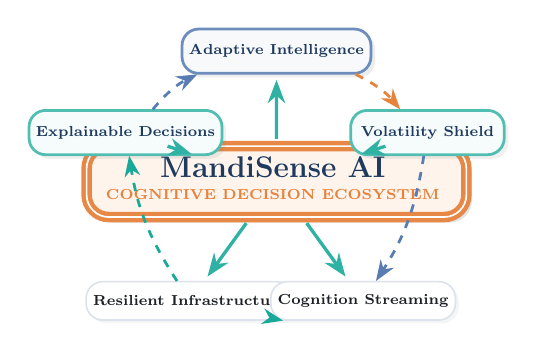
\begin{tikzpicture}[scale=0.72, every node/.style={scale=0.75}]
  % Central Hub
  \node[cardHighlight, minimum width=4.5cm, minimum height=1.2cm, double, draw=accentOrangeDark!95] (hub) at (0,0) {
    \begin{tabular}{c}
      \bfseries\Large MandiSense AI \\
      \fontsize{7}{8}\selectfont\color{accentOrangeDark}\bfseries COGNITIVE DECISION ECOSYSTEM
    \end{tabular}
  };
  
  % Surrounding Nodes
  \node[cardPrimary, minimum width=2.6cm] (adaptive) at (90:2.3cm) {Adaptive Intelligence};
  \node[cardTeal, minimum width=2.6cm] (explain) at (162:2.8cm) {Explainable Decisions};
  \node[cardNode, minimum width=2.6cm] (resilient) at (234:2.6cm) {Resilient Infrastructure};
  \node[cardNode, minimum width=2.6cm] (cognition) at (306:2.6cm) {Cognition Streaming};
  \node[cardTeal, minimum width=2.6cm] (shield) at (18:2.8cm) {Volatility Shield};

  % Bidirectional and directional connections
  \draw[flowArrowAccent] (hub) -- (adaptive);
  \draw[flowArrowAccent] (hub) -- (explain);
  \draw[flowArrowAccent] (hub) -- (resilient);
  \draw[flowArrowAccent] (hub) -- (cognition);
  \draw[flowArrowAccent] (hub) -- (shield);
  
  % Circular flows showing integration with color matching!
  \draw[->, >=Stealth, dashed, line width=1.0pt, accentOrangeDark, bend left=12] (adaptive) to (shield);
  \draw[->, >=Stealth, dashed, line width=1.0pt, primary!80, bend left=12] (shield) to (cognition);
  \draw[->, >=Stealth, dashed, line width=1.0pt, accentTeal, bend left=12] (cognition) to (resilient);
  \draw[->, >=Stealth, dashed, line width=1.0pt, accentTeal, bend left=12] (resilient) to (explain);
  \draw[->, >=Stealth, dashed, line width=1.0pt, primary!80, bend left=12] (explain) to (adaptive);
\end{tikzpicture}
\vspace{0.05cm}
\begin{columns}[T]
  \column{0.32\textwidth}
  \begin{smallcard}[\linewidth]
    \centering\scriptsize\bfseries\color{primaryDark} 1. Operational Cognition\\
    \tiny\color{textMedium} Real-time volatility regime detection dynamically gates prediction weights, shielding clients from outliers.
  \end{smallcard}
  \column{0.32\textwidth}
  \begin{smallcard}[\linewidth]
    \centering\scriptsize\bfseries\color{accentTeal} 2. Trustworthy Explanations\\
    \tiny\color{textMedium} Live SHAP feature contributions are coupled with action-oriented advisory descriptions, driving operator confidence.
  \end{smallcard}
  \column{0.32\textwidth}
  \begin{smallcard}[\linewidth]
    \centering\scriptsize\bfseries\color{accentOrangeDark} 3. Keynote Infrastructure\\
    \tiny\color{textMedium} High-concurrency async pipelines achieve sub-200ms p95 latency, backed by Prometheus self-healing operations.
  \end{smallcard}
\end{columns}
\end{frame}

% --- SLIDE 17: THANK YOU ---
{
\setbeamercolor{background canvas}{bg=white}
\begin{frame}[plain]
\vspace{2cm}
\centering
{\color{primaryDark}\Huge\bfseries Thank You}
\vspace{0.5cm}
{\color{primary}\rule{0.25\textwidth}{1pt}}
\vspace{0.5cm}
{\LARGE\color{textMedium}Questions \& Discussion}
\vspace{1.5cm}
{\Large\color{textLight}MandiSense AI · IEEE/ACM Conference on AI Systems Engineering · 2026}
\end{frame}
}

\end{document}